\documentclass{article}
\usepackage{amsmath}
\usepackage{amssymb}
\usepackage{empheq}
\usepackage{cancel}
\usepackage{hyperref}
\usepackage[most]{tcolorbox}
\usepackage{verbatim}
\usepackage{pgfplots}
\usepackage{pgf,tikz}
\usepackage{geometry}
\geometry{a4paper, total={170mm,257mm},
           left=20mm, top=20mm }

\usetikzlibrary{positioning, patterns}
\usetikzlibrary{decorations.pathmorphing}
\usetikzlibrary{arrows.meta, shadows, shapes.symbols}
\graphicspath{ {./images/} }
%%\pgfplotsset{compat=1.15}

\newcommand{\pder}[2]{\frac{\partial #1}{\partial #2}}
\newcommand{\pders}[2]{\frac{\partial^2 #1}{{\partial #2}^2}}
\newcommand{\fe}{f + \epsilon \eta}
\newcommand{\fep}{f^\prime + \epsilon \eta^\prime}

\newcommand{\PHI}{\phi\lb f, f^\prime, x \rb}
\newcommand{\PHIe}{\phi\lb fe, \fep, x \rb}
\newcommand{\delFfEta}{\left < \nabla F_f \: , \eta \right >} 
\newcommand{\delxFfEta}{\left < \nabla^2 F_f \: , \eta \right >} 

\newcommand{\lb}{\left(}
\newcommand{\rb}{\right)}
\newcommand{\lcb}{\left\{}
\newcommand{\rcb}{\right\}}
\newcommand{\lsb}{\left[}
\newcommand{\rsb}{\right]}

\begin{document}

\title{On determination of function extrema with MaxEnt formulation}
\author{Ravi Sankar Saripalli}

\maketitle

\begin{tcolorbox}[fonttitle=\sffamily\bfseries\large,
                  title=Description]

                  This is an attempt to find extrema of a function 
                  with MaxEnt formulation. The usual way to
                  find extrema of a function $f(x)$  is to find $x$ where function
                  derivative $f^\prime (x)$ vanishes. An alternate approach is to use probability distribution function
                  $p(x)$ as an independant parameteric function and seek to maximize the expected value of $f(x)$ based on the
                  $p(x)$ with the condition that entropy (as defined by Shanon) of the probability distribution $p(x)$ is maximized, thus
                  ensuring that the distribution function derived is least biased.

\end{tcolorbox}
\begin{tcolorbox}[fonttitle=\sffamily\bfseries\large,
                  title=The MaxEnt Lagrangian]

%% Equation 1
\begin{empheq}[box=\tcbhighmath]{equation}
  \begin{split}
       \mathcal{L} (p, \lambda ) = \int f(x) p(x) dx 
                                    + T  \int p(x) ln(p(x)) dx 
                                    + \lambda \left \{ \left ( \int p(x) dx \right ) - 1 \right \}  
  \end{split}
\end{empheq}

    The first term in the Lagrangian is the expected value of the function corresponding to the PDF $p(x)$,
    the second term corresponds
    to the entropy of the PDF scaled by an arbitray constant $T$ and the last  term corresponds to the equality 
    constraint that integral of PDF is one. The multiplier $\lambda$ is the Lagrangian parameter.
\\
    Noting that the Lagrangian is function of $p(x)$ and $\lambda$,  the extrema of the Lagrangian is obtained
    by requiring the functional derivative with respect $p(x)$ and the Lagrangian parameter $\lambda$ are zero.
    
    Although this enables us to determine $p(x)$ and $\lambda$ corresponding to the extrema, we need additional
    criterion to determine if the extrema is either 
    minimum or maximum. Sign of the second derivative in functional space 
    similar to simple variables can be used to ascertain if the stationary point corresponds to minima or maxima.


\end{tcolorbox}

\begin{tcolorbox}[fonttitle=\sffamily\bfseries\large,
                  title=The Euler-Lagrange equation]

Consider the following functional (function of functions)
%% Equation 2
\begin{empheq}[box=\tcbhighmath]{equation}
  \begin{split}
      & F \lb f^{\prime}, f, x \rb = \int \phi \left ( f^{\prime} (x), f(x), x \rb dx  
  \end{split}
\end{empheq}

  Requiring that functional derivative of $F$ with respect to $f$ is zero at extrema  
 (note $f$ is a function not a variable, hence 
   the name functional derivative) following Eauler-Lagrange  equation can be derived.

%% Equation 3
\begin{empheq}[box=\tcbhighmath]{equation}
       \frac{\partial \phi}{\partial y}
          - \frac{d}{dx}\lb \frac{\partial \phi}{\partial y^\prime} \rb = 0 
\end{empheq}
    \text{Derivation of the above equation that is easy to follow is  
    \href{https://farside.ph.utexas.edu/teaching/336L/Fluid/node266.html}{here}}

\end{tcolorbox}


\begin{tcolorbox}[fonttitle=\sffamily\bfseries\large,
                  title=Finding Stationary Point of Lagrangian in Eq 1.]

Using the above Euler-Lagrange equation, the stationary conditions for the Lagrangian in equation 1, 
can be derived from functional derivative with respective $p$ and the 
derivative with respective $\lambda$ as follows.

%%Equation 4
\begin{empheq}[box=\tcbhighmath]{equation}
  \begin{split}
      & f(x) + T \lcb 1  + ln(p(x)) \rcb + \lambda = 0
  \end{split}
\end{empheq}

%%Equation 5
Setting derivative with respect to $\lambda$ to zero yields the contraint that PDF integral should be 1.
\begin{empheq}[box=\tcbhighmath]{equation}
  \begin{split}
      & \int p(x) \:  dx  - 1 = 0  
  \end{split}
\end{empheq}

%%Equation 6
Rearranging eqn.4 
\begin{empheq}[box=\tcbhighmath]{equation}
  \begin{split}
      &  p(x) =  e^{ -\lb 1 + \lambda / T  \rb }   \: e^{-f(x)/T}
  \end{split}
\end{empheq}

Combining eqns. 5 and 6 the value of lambda can be expressed as follows
\begin{empheq}[box=\tcbhighmath]{equation}
  \begin{split}
      &  \lambda = T \lcb ln \int e^{-f(x)/T} dx  - 1 \rcb
  \end{split}
\end{empheq}

    The question to ask is how do we now proceed to get min or max of $f(x)$ given that we have it
    in analytical form (eg. sin(x)).. What will be the p(x) as T approaches zero. That is the intent
    of the annealing process as we converge on p(x).
\end{tcolorbox}

\begin{tcolorbox}[fonttitle=\sffamily\bfseries\large,
                   title=Explorations with sinx ]
  Assuming that we are interested in finding extrema of sin(x) in the interval $[0,\pi]$,
  one can proceed as follows.
  \begin{enumerate}
     \item {For a given T, calculate $\lambda$ by evaluating the integral numerically}
     \item {With $T and \lambda$ known, the PDF $p(x)$ now is well defined (eq.6). The expected value of $f(x)$ can be
       determined by numerical integration of $\int p(x) f(x) dx$ }
  \end{enumerate}
 
\end{tcolorbox}

\begin{tcolorbox}[fonttitle=\sffamily\bfseries\large,
  title={$sin(x)$} ]
    \centering
     %% Generates x) plot between 0 and pi
  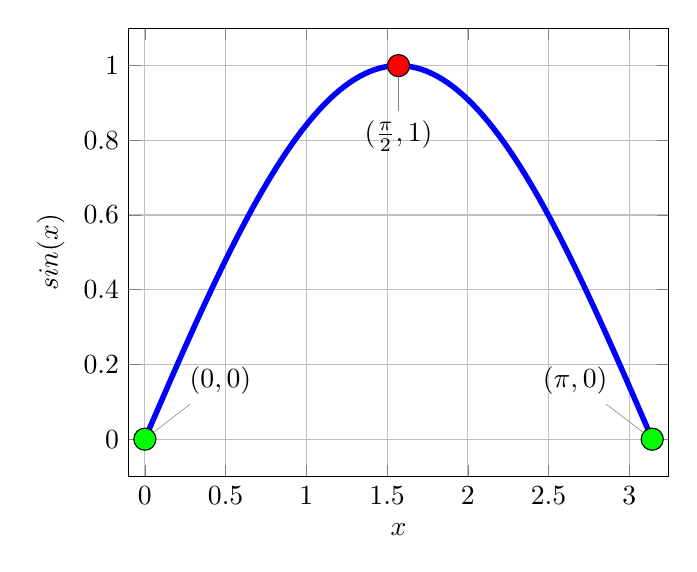
\begin{tikzpicture}
    \begin{axis}[ xlabel = $x$,
	  ylabel = {$sin(x)$},
	  ymin = -0.1, ymax = 1.1,
	  xmin = -0.1, xmax = pi + 0.1,
	  grid=both,
	  domain = 0:pi
	]
       \addplot[color=blue, line width=2pt, samples=100] 
          {sin(x*180/pi)} ;
       \addplot[only marks, mark options={fill=green,scale=2} ]
          coordinates { (0,0) (pi, 0) } ;
       \addplot[only marks, mark options={fill=red,scale=2} ]
	  coordinates { (pi/2, 1) };
	  
	  \node[pin=270:{$(\frac{\pi}{2}, 1)$}] at (axis cs:pi/2,1) {} ;
	  \node[pin=45:{$(0,0)$}] at (axis cs:0,0) {} ;
	  \node[pin=135:{$(\pi,0)$}] at (axis cs:pi,0) {} ;
    \end{axis}
  \end{tikzpicture}

\end{tcolorbox}

\begin{tcolorbox}[fonttitle=\sffamily\bfseries\large,
  title=Change in pdf with T when $T \le 0$ and $T \ge 0$ ]
     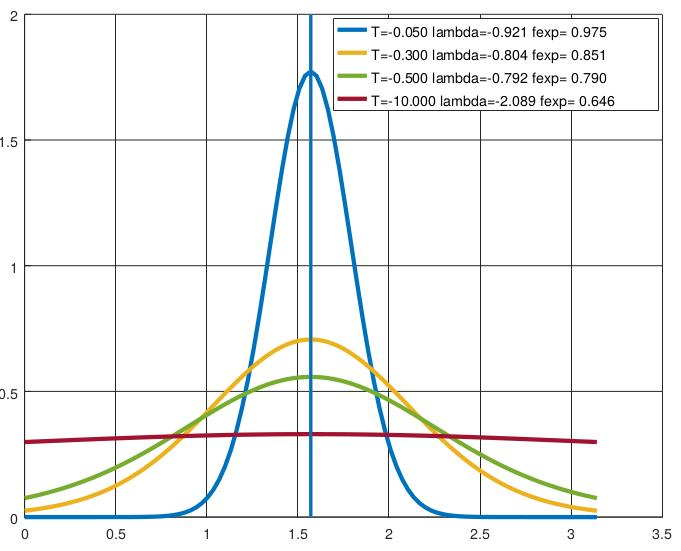
\includegraphics[scale=0.25]{fig1.jpg}
     \hspace{1cm}
     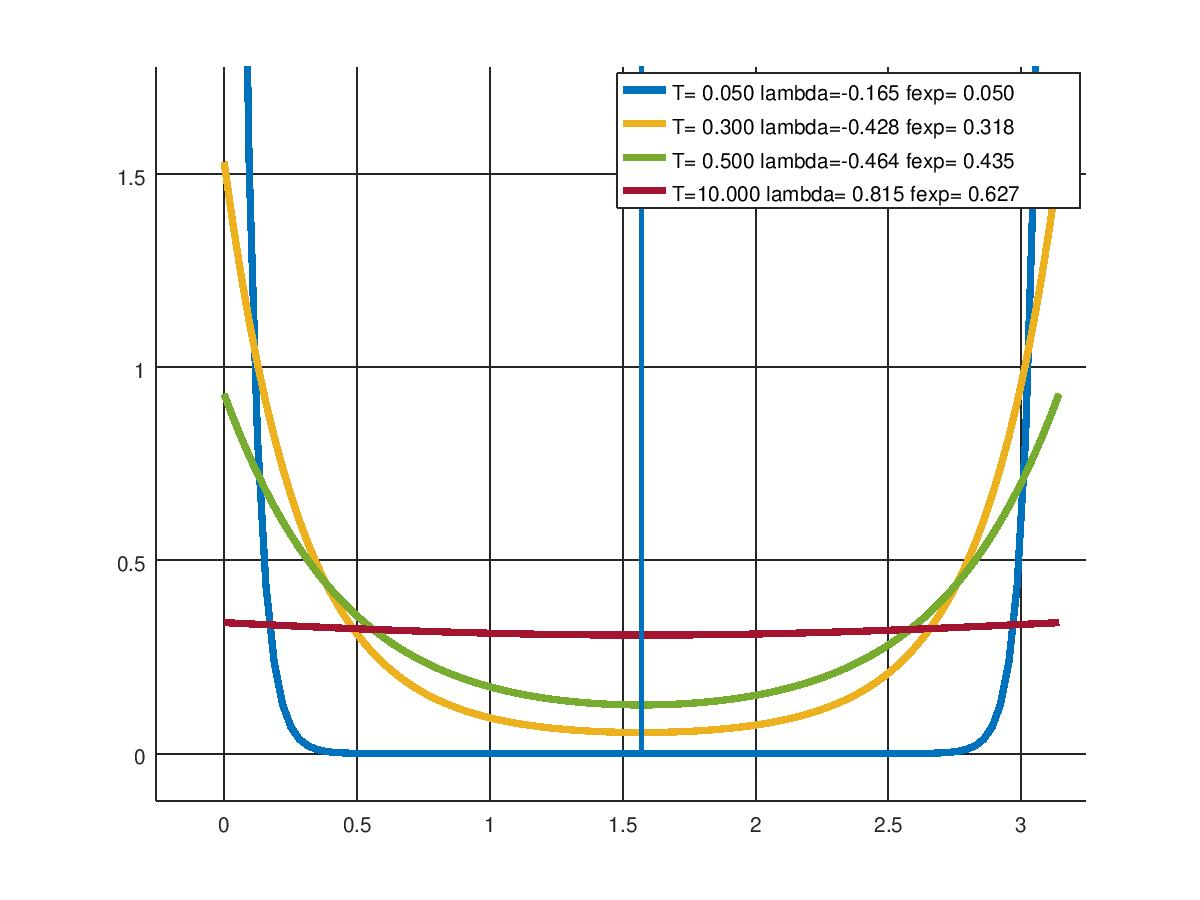
\includegraphics[scale=0.32]{fig2.jpg}
\end{tcolorbox}


From the above figures, it is clear that for $T \ge 0$ as its 
magnitude approaches zero, the pdf spread decreases and
tends to peak around the true maxima. On the otherhand,
when $T \ge 0$, the pdf peaks appear near the end points where
the function has minimal value in the interval of interest. 

Let us now explore a different function that has two peaks, and trough as shown in the
following figure. 
\begin{tcolorbox}[fonttitle=\sffamily\bfseries\large,
    title={$y(x)=8(1-2x^2)x^2  -0.6<x<0.6  $} ]
    \centering
     %% Generate 8*(1-2*x^2)*x^2
%%  between x=-0.6 to 0.6

  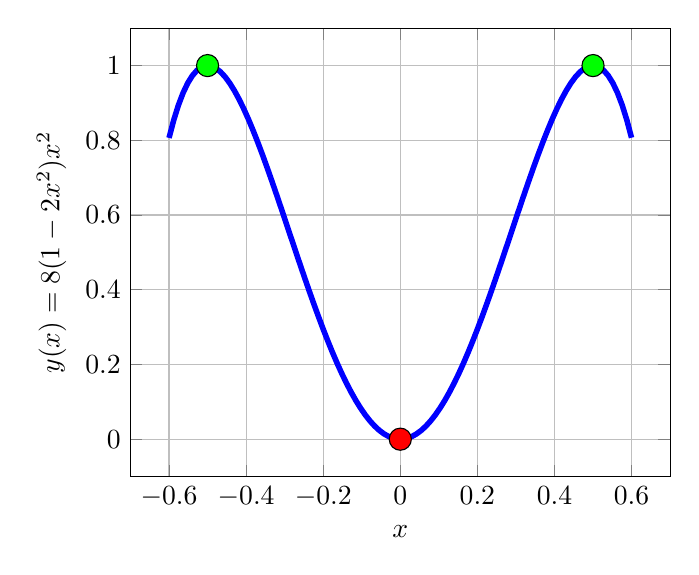
\begin{tikzpicture}
    \begin{axis}[ xlabel = $x$,
        ylabel = {$y(x)=8(1-2x^2)x^2$},
	  ymin = -0.1, ymax = 1.1,
	  xmin = -0.7, xmax = 0.7,
	  grid=both,
	  domain = -0.6:0.6
	]
       \addplot[color=blue, line width=2pt, samples=100] 
	  {8*(1-2*x*x)*x*x)} ;
          
       \addplot[only marks, mark options={fill=green,scale=2} ]
          coordinates { (-0.5, 1) (0.5, 1) } ;
       \addplot[only marks, mark options={fill=red,scale=2} ]
	  coordinates { (0,0) };
	  
	  
    \end{axis}
  \end{tikzpicture}

\end{tcolorbox}

Using the above function, the effect of $T$ on PDF corresponding to the stationary
point is determined as described earlier.

\begin{tcolorbox}[fonttitle=\sffamily\bfseries\large,
    title=Effect of $T$ on PDF at stationary condition]
     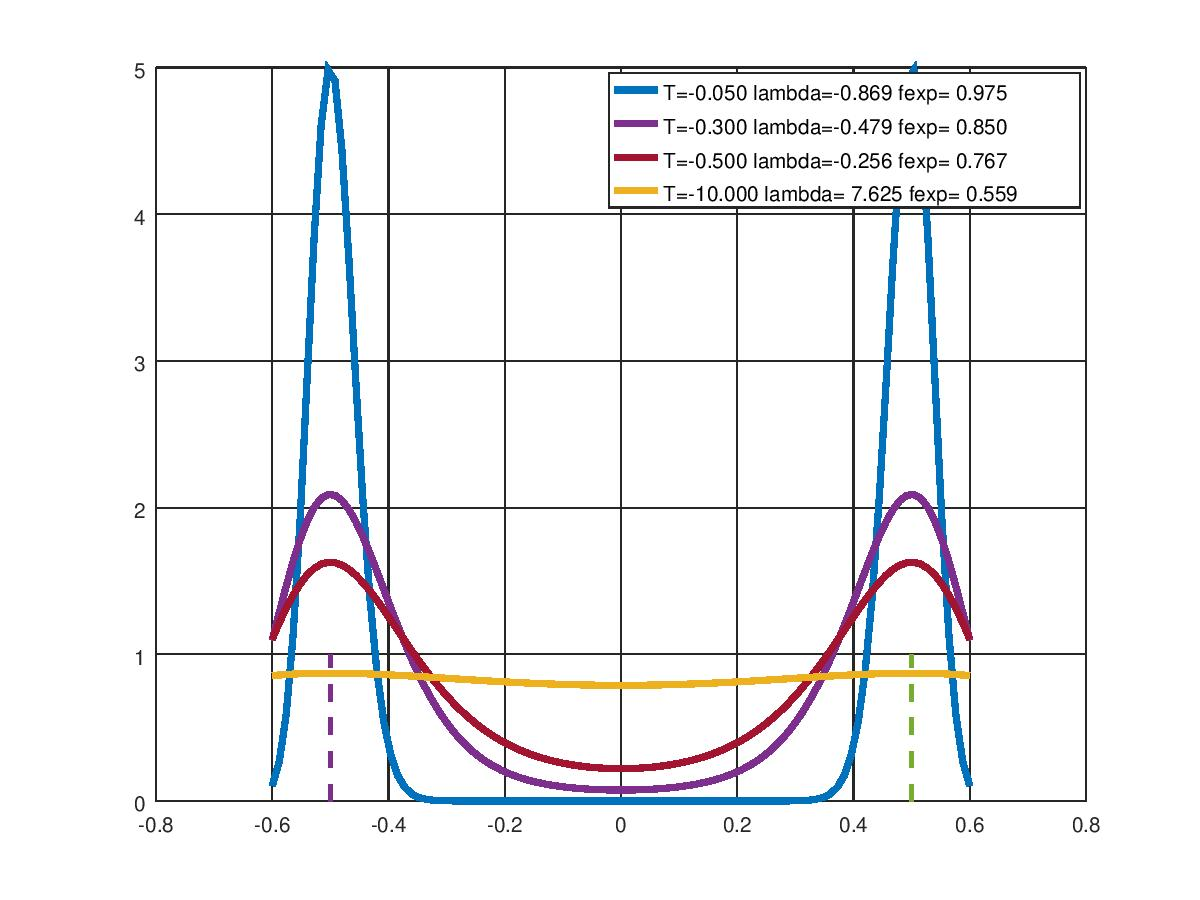
\includegraphics[scale=0.3]{fig3.jpg}
     \hspace{1cm}
     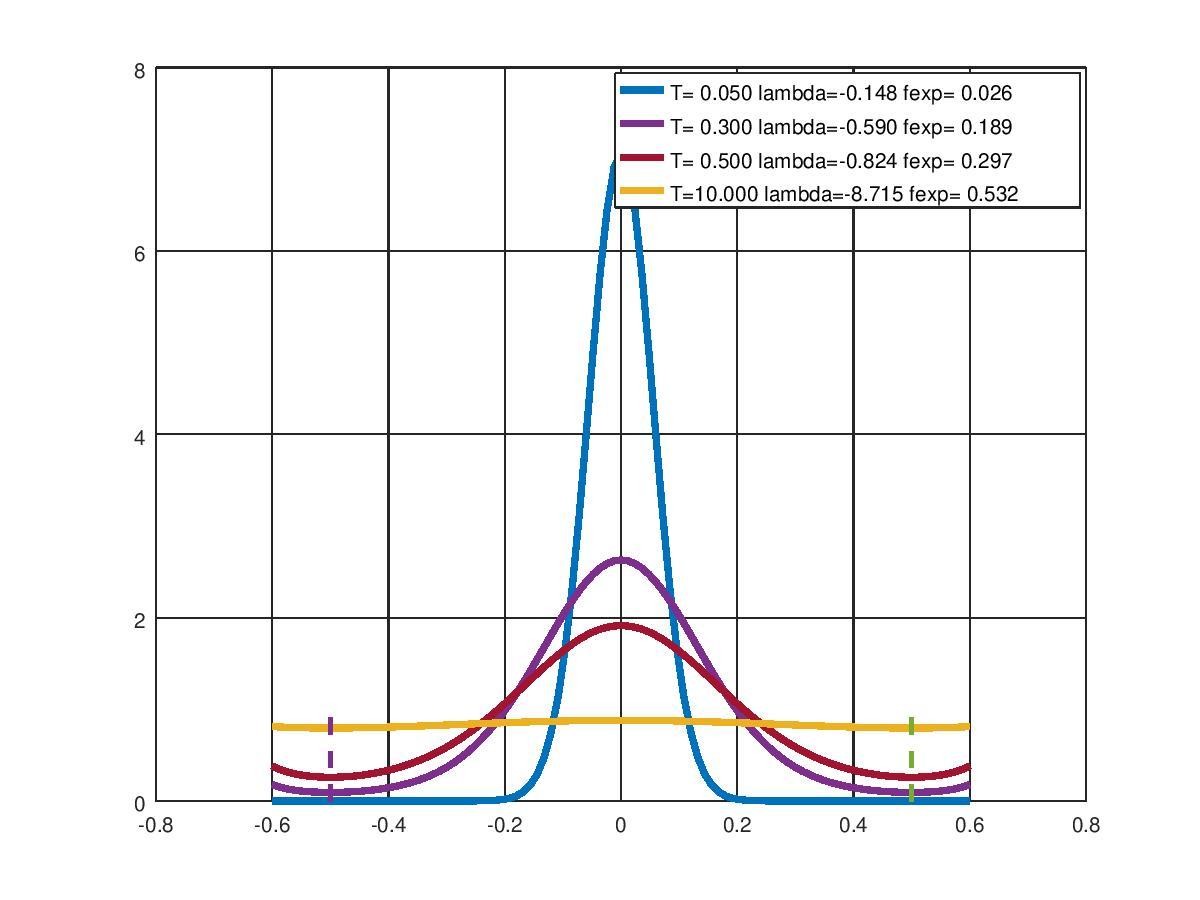
\includegraphics[scale=0.3]{fig4.jpg}
\end{tcolorbox}

Once again, when $T$ value is approaching zero from positive side,
the PDF corresponding to extrema condition peaks around the true minima
at $x=0$ with corresponding expected value of function approaching 0.
When $T$ approaches zero from the negative side, the PDF peaks around
$x=-0.5, and 0.5$ with expected value of function approaching 1.

It therefore appears that when $T$ approaches zero from negative side
PDF determined from stationary condition corresponds to maxima of the function,
while it approaches zero from positive side, the PDF peaks around the minima of the 
function.




\begin{tcolorbox}[fonttitle=\sffamily\bfseries\large,
                  title={Functional Derivatives} ]
In this section the derivation of functional derivatives 
is provided. While there is no shortage of articles on this topic,
thesis work by 
\href
    {http://www-users.math.umn.edu/~olver/ln_/cv.pdf}{Peter J. Oliver} from University of Minnesota.
provides lucid explanation.

    Let $\eta(x)$ be an arbitrary function which vanishes to zero at the boundaries, and 
    $\epsilon$ is an arbitrarily small constant. For the functional $F$ defined in equaiton 2,
    we denote its gradient with respect to $f(x)$ with
    $\nabla F_f$, and $\eta(x)$ is the variation of function $f(x)$, then

\begin{empheq}[box=\tcbhighmath]{equation}
  \begin{split}
      & \delFfEta = \frac{d}{d\epsilon} F\lb\fe\rb \Bigr\rvert_{\epsilon=0} \\
      & \text{where} \\     
      & \left < \nabla F_f, \eta \right > = \int \nabla F_f \eta (x) dx 
  \end{split}
\end{empheq}

\begin{equation*}
  \begin{split}
      \delFfEta  &=  \frac{d}{d \epsilon} \int  {\PHIe} dx  \Bigr\rvert_{\epsilon=0} \\
                 &= \int \lcb
                    \eta \pder{\PHIe}{\lb\fe\rb}
                   + \eta^\prime \pder{\PHIe}{\lb\fep\rb}
                   \rcb dx
                   \Bigr\rvert_{\epsilon=0} \\
                 &= \int \lcb
                    \eta \pder{\PHI}{f}
                  + \eta^\prime  \pder{\PHI}{f^\prime}
                 \rcb dx \\ 
                 &= \int  \eta \pder{\PHI}{f} dx 
                    + \cancelto{0}{\Bigg[\eta \pder{\PHI}{f} \Bigg]_{a}^{b}} 
                    - \int  \eta \frac{d}{dx} \lcb \pder{\PHI}{f^\prime} \rcb dx  \\
                 &= \int  \eta \Bigg[
                                   \pder{\PHI}{f}  -
                                    \frac{d}{dx} \lcb \pder{\PHI}{f^\prime} \rcb 
                      \Bigg] dx 
  \end{split}              
\end{equation*}

     Since $\eta(x)$ is arbitray function
     
\begin{empheq}[box=\tcbhighmath]{equation}
  \begin{split}
      \nabla F_f = \pder{\PHI}{f}  
                   - \frac{d}{dx} \lcb \pder{\PHI}{f^\prime} \rcb
  \end{split}
\end{empheq}

Similarly the second variation of $f$ can be defined and evaluated as follows.
It should be noted that unlike, the first variation, it is not possible to 
eliminate $\eta\prime$ through integration by parts.

\begin{empheq}[box=\tcbhighmath]{equation}
  \begin{split}
    Q(f,\eta) &= \frac{d^2}{d\epsilon^2} F\lb\fe\rb \Bigr\rvert_{\epsilon=0} \\
                 &= \int \lcb
                    \eta^2 \pders{\phi}{f}
		  + \lb\eta^\prime\rb^2  \pders{\phi}{f^\prime}
		  + 2 \eta \eta^\prime \frac{\partial^2{\phi}}
				            {\partial{f}\partial{f^\prime}}
		  \rcb dx
   \end{split}
\end{empheq}

Similar to normal functions, the sign of the second variation can be used to ascertain if the stationary point of the functional corresponds to either maxima or minima.
If $Q(f,\eta)$ is positive definite at the stationary point then it is minima.

One way $Q(f,\eta)$ can be positive definite is when the integrand itself is positive definite over the entire integration interval. While that is a valid possibility, it is too prescriptive.

\end{tcolorbox}

\begin{tcolorbox}[fonttitle=\sffamily\bfseries\large,
  title={Necessary and sufficient conditions for second functional positivity} ]
Expressing $Q(f,\eta)$ as follows

\begin{equation*}
  \begin{split}
    Q(f,\eta)   &= \int \lcb A  \eta^2 
		                  + 2 B \eta \eta^\prime 
		                  + C \lb\eta^\prime\rb^2  
		          \rcb dx \\
     & where \:\:  
		    A =  \pders{\phi}{f}  \:;\:  
		    B =  \frac{\partial^2\phi}{\partial f\partial {f^\prime}} \:;\:  
		    C =  \pders{\phi}{f^\prime}  \\
     &= \int \lcb A \eta^2 + B \frac{d}{dx}\lb\eta^2\rb    
		                  + C \lb\eta^\prime\rb^2  
		          \rcb dx \\
     &= \int \lcb A \eta^2 - B^\prime \eta^2
		                  + C \lb\eta^\prime\rb^2  
 	      \rcb dx  \:\:  
  \end{split}
\end{equation*}
Nb: The last simplification is achieved with integration by parts and  noting $\eta$ vanishes on boundaries

The necessary and sufficient conditions for $Q(f,\eta)$ to be positive requires fairly involved mathematics and is nicely covered in text book (page 100-110) on \href{https://epdf.pub/calculus-of-variations3a9621c1bc7c0b0a7e6500c574abb0e427979.html}{Variational Calculus}
The two necessary conditions for second variant to be positive definite are as follows.
\begin{empheq}[box=\tcbhighmath]{equation}
  \begin{split}
    \text{Condition 1:} & \\
    & C > 0      \\
    \text{Condition 2:} & \\
    &\text{The following linear differential has} \\
    & \text{no other solution but a trivial solution $v=0$} \\
    &	   - \frac{d}{dx} \lb C \eta^\prime \rb  + 
	   \lb A - B^\prime \rb \eta = 0
   \end{split}
\end{empheq}
\end{tcolorbox}


\begin{tcolorbox}[fonttitle=\sffamily\bfseries\large,
    title={The role of sign of scaling parameter T in equation (1) explained} ]
Referring back to our original Lagrangian in equation 1 the second variation can be calculated as follows.
\begin{equation*}
    \begin{align}
        Q(p,\eta) & = \lim_{\epsilon \to 0}  \frac{d^2}{d\epsilon^2} 
                 \begin{cases}
                 \begin{rcases}
                     \begin{split}
                     & \int f(x) \lcb p(x)+\epsilon \eta(x) \rcb dx
                           + T \int  \lcb p(x) + \epsilon \eta(x) \rcb 
                              ln \lcb p(x)  + \epsilon \eta(x) \rcb dx \\ 
                         &\qqad\qquad  + \int \lcb p(x)+\epsilon \eta(x) \rcb
                         dx \rcb  
                     \end{split}
                 \end{rcases}
                 \end{cases}
                   \\ & = \lim_{\epsilon \to 0} \frac{d}{d\epsilon} 
                  \lcb \int f(x) \eta(x) dx
                         + T \int   \eta(x) \lsb 
                          ln \lcb p(x)  + \epsilon \eta(x) \rcb  + 1 \rsb dx 
                         +    \int \eta(x) dx \rcb \\
                  & =  T * \int \frac{\eta^2(x)}{p(x)} dx   
    \end{align}
\end{equation*}

    From the above derivation it is clear that sign of the  second variation of the Lagrangian of our interest (Eq. 1)
    is same as that of $T$ 
    because $p(x)$ and $\eta^2$ are always positive. This explains our observed trends (with few sample functions)
    where stationary points tunred out to be minima when T is positive, and maxima when T is positive.
    Since the above derivation is valid for any generic function $f(x)$ we can use this result to seek either maxima
    or minima for the MaxEnt problem by appropriate choice of sign for T.
\end{tcolorbox}


\begin{tcolorbox}[fonttitle=\sffamily\bfseries\large,
    title={Distributed MonteCarlo Tree Search Algorithm} ]
\begin{empheq}[box=\tcbhighmath]{equation}
  \begin{split}
      \mathcal{L}\lb q_i, \lambda_i \quad  i=1..N\rb & =
           \int G(x_1, x_2, ... x_N) \prod_{i=1}^{N} q_i(x_i) \quad dx_1 dx_2 .. dx_N
          \\ & + T \sum_{i=1}^{N} \int q_i(x_i) ln(q_i(x_i)) dx_i 
          \\ & + \sum_{i=1}^{N}\lambda_i \lcb \lb \int q(x_i) dx_i \rb - 1  \rcb 
  \end{split}
\end{empheq}

The above Lagrangian is formed to enable minimise the global objective function $G$ which is a function of all the
variables $x_1, x_2 ... x_N$. The probability distribution function (PDF) of each agent is represneted by $q_i(x_i)$.
It is assumed that the approximate collective PDF can be represented as product of distribution functions of each agent. This
assumption enables decentralization of each agents actions while allowing optimization of the global objective function $G$.
    The stationary conditions for  Lagrangian in eqn. 12 with respect of $q_k(x_k)$ and $\lambda_k$ can be written as follows.

\begin{empheq}[box=\tcbhighmath]{equation}
  \begin{rcases}
  \begin{split}
      \nabla_{q_k}\mathcal{L} &=
        \int G(x_1, x_2, ... x_N) \prod_{i \ne k} q_i(x_i) \quad \prod_{i \ne k} dx_i
           + T \lcb  1 +  ln(q_k(x_k)) \rcb 
           + \lambda_k  \\
        & =  E(G|x=x_k) 
           + T \lcb  1 +  ln(q_k(x_k)) \rcb 
           + \lambda_k  = 0 \\
      \nabla_{\lambda_k}\mathcal{L} &=
            \lcb \lb \int q(x_k) dx_k \rb - 1  \rcb = 0 
  \end{split}
  \end{rcases} _{k=1..N}
\end{empheq}
The Lagrangian parameter $\lambda_k$ can be elemenated from the above two conditions
and it is trivial show that 
\begin{empheq}[box=\tcbhighmath]{equation}
    q_k(x_k) = \frac{e^{-E(G|x=x_k)/T}}{\int e^{-E(G|x=x_k)/T} dx_k} 
\end{empheq}
\end{tcolorbox}


\begin{tcolorbox}[fonttitle=\sffamily\bfseries\large,
    title={Newton method to minimize Lagrangian based on collective probability $p(x)$} ]

    In this seciton the iteration scheme to find the stationary point with respect to $p(x)$
    to the Lagrangian in equation 1
    is derived based on Newton method. The Newton iteration template for any arbitray function $f(x)$ 
    is $x_{new} = x_0 - \frac{\nabla f(x_0)}{\nabla^2 f(x_0)}$. Although this example is based on 
    normal functions, it appears that one can use this strategy in functional space ???. 

    The first and second
    variations of the Lagrangian of interest have already been derived. Althogh these are integral expressions, 
    choosing the arbitray function $\eta$ to be a delta function $\delta(x=x^\prime)$ the point wise first 
    and second derivatives of the functional can be realized. (This statement needs some review ... by mathematician for 
    rigour)
\begin{empheq}[box=\tcbhighmath]{equation}
  \begin{split}
      \nabla_p\mathcal{L} |_{p=p^0} &=  f(x) + T \lcb 1 + ln(p^0(x)) \rcb + \lambda \\   
      \nabla_p^2\mathcal{L} |_{p=p^0} &=   \frac{T}{p^0(x)}  \\   
      p^{new}(x) &= p^0(x) - \frac { f(x) + T \lcb 1 + ln(p^0(x)) \rcb + \lambda  }
                                  { \frac{T}{p^0(x)} }    \\   
      p^{new}(x) &= - p^0(x) \lcb     \frac{f(x)}{T}  + ln(p^0(x)) + \frac{\lambda}{T} \rcb \\
      &\text{Integrating over the domain and noting that $\int p^{new}(x)dx = 1 \text{;} $\int p^0(x) dx =1$} \\
      1 &= - \frac{1}{T} \int p^0(x)f(x) dx - \int p^0(x) ln(p^0(x)) dx - \frac{\lambda}{T} \\
      & \text{The $\lambda$ value can now be expressed as follows} \\
      \lambda &= -T -  \int p^0(x)f(x) dx - T \int p^0(x) ln(p^0(x)) dx  =  -T - E(f,p^0) + T S(p^0) \\
      &\text{Finally the $p_{new}$ can now be written as} \\
      p^{new}(x) &= - p^0(x) \lcb     \frac{f(x)}{T}  + ln(p^0(x)) - 1 - \frac{1}{T} E(f,p^0) +S(p^0)   \rcb \\
      \frac {p^{new}(x)}{p^0(x)} &=   1 - S(p^0) - ln(p^0(x)) - \frac{1}{T} \lcb f(x) - E(f,p^0) \rcb \\
  \end{split}
\end{epheq}
\end{tcolorbox}

\end{document}
